\documentclass[../discrete.tex]{subfiles}
\graphicspath{{\subfix{../figures/}}}
\begin{document}
\chapter{Logic and Proofs}
\section{Propositional Logic}
A proposition is a declarative statement that is either true or false, but not both. We use letters to denote propositional variables. 
The conventional letters for propositional variables are $p,q,r,s$. True is notated as T and false is notated as F. An atomic proposition 
is a proposition that cannot be expressed in terms of simpler propositions.
\begin{definition}
    Let $p$ be a proposition. The negation of $p$, denoted by $\neg{p}$ (or $\bar{p}$) means "It is not the case that $p$".

    The proposition $\neg{p}$ is read as "not $p$". The truth value of the negation of $p$, $\neg{p}$ 
    is the opposite of the truth value of $p$.
\end{definition}

The negation of a proposition can also be considered the result of the operation of the negation operator on a proposition. 

The next operator is a connective and it is used to form new propositions from two or more existing propositions.
\begin{definition}
    Let $p$ and $q$ be propositions. The conjunction of $p$ and $q$, denoted by $p\land q$, 
    is the proposition of "$p$ and $q$". The conjunction $p\land q$ is true when both are true, and false when both are false.
\end{definition}

\begin{definition}
    Let $p$ and $q$ be propositions. The disjunction of $p$ and $q$, denoted by $p\lor q$, 
    is the proposition "$p$ or $q$". The disjunction $p\lor q$ is false when both $p$ and $q$ are false, otherwise it is true.
\end{definition}

\begin{definition}
    Let $p$ and $q$ be propositions. The exclusive or of $p$ and $q$, denoted by $p\oplus{q}$ 
    is the proposition that is true when exactly one of $p$ and $q$ is true and is false otherwise.
\end{definition}

There are other ways propositions can be combined.
\begin{definition}
    Let $p$ and $q$ be propositions. The conditional statement $p\rightarrow q$, is 
    the proposition, "if $p$, then $q$". The conditional statement $p\rightarrow q$ is 
    false when $p$ is true and $q$ is false, and true otherwise. $p$ is called the 
    hypothesis and $q$ is called the conclusion.
\end{definition}

A conditional statement is also called an implication.

With $p\rightarrow q$, we can form three related conditional statements. 

The first is the proposition $q\rightarrow p$, which is the converse of $p\rightarrow q$. 

The contrapositive of $p\rightarrow q$ is $\neg q\rightarrow \neg p$.

The inverse of $p\rightarrow q$ is $\neg p \rightarrow \neg q$.

The contrapositive of a conditional statement is equal to it. We all two compound propositions 
equivalent when they always have the same truth values. The converse and inverse of a conditional 
statement are equivalent as well.

There is another way to combine propositions that expresses that two propositions have the same truth value.
\begin{definition}
    Let $p$ and $q$ be propositions. The biconditional statement $p\leftrightarrow q$ 
    is the proposition "$p$ if and only $q$". This statement is true if $p$ and $q$ have 
    the same truth values, and is false otherwise.
\end{definition}

The negation operator is applied before all logical operators. Another general rule is 
that the conjunction operator takes precendence over the disjunction operator. It is an accepted 
rule that conditional and biconditional operators have lower precendence than the conjuction and disjunction operators. 

A bit is a symbol with two values, 0 and 1. 1 is true, and 0 is false. 

\section{Propositional Equivalences}
\begin{definition}
    A compound proposition that is always true, no matter what the truth values of the 
    propositional values that occur in it, is called a tautology. A compound proposition that is 
    always false is called a contradiction. If it is neither a tautology or a contradiction, it is called a contingency.
\end{definition}

Compound propositions that have the same truth values in all possible cases are called logically equivalent. 
\begin{definition}
    The compound propositions $p$ and $q$ are called logically equivalent if $p\leftrightarrow q$ is a 
    tautology. The notation $p\equiv q$ denotes that $p$ and $q$ are logically equivalent.
\end{definition}

We can establish logical equivalence of more than two compound propositions. Generally $2^n$ 
rows are required if a compound proposition involves $n$ propositional variables.
\begin{center}
    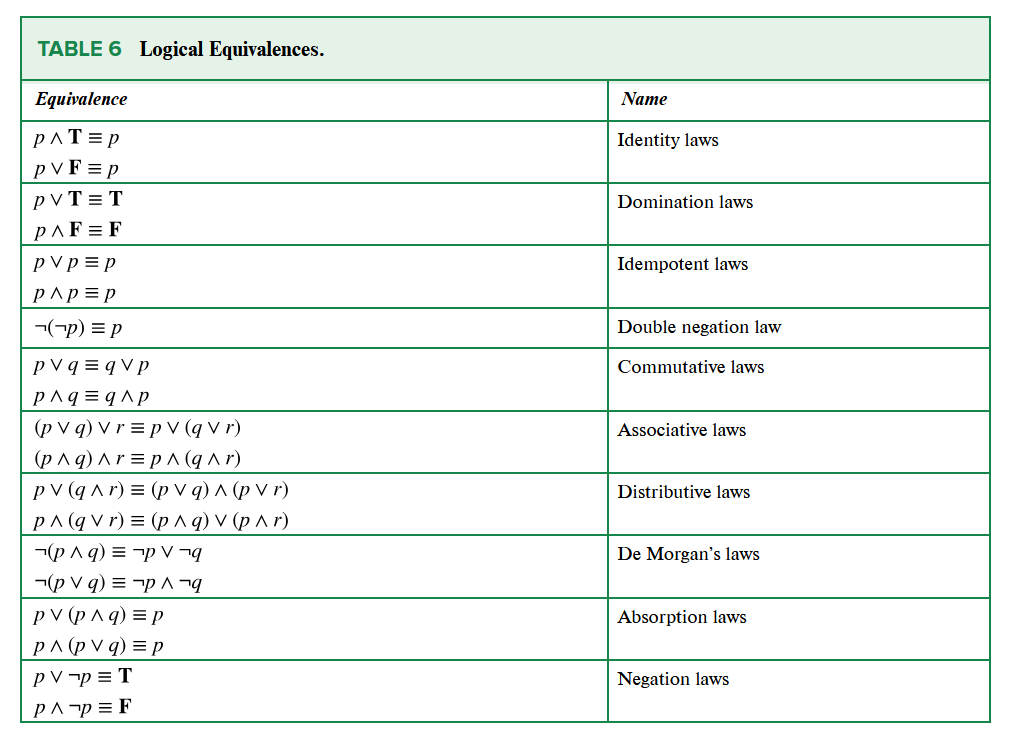
\includegraphics[width=0.72\textwidth]{1.3D.PNG}
    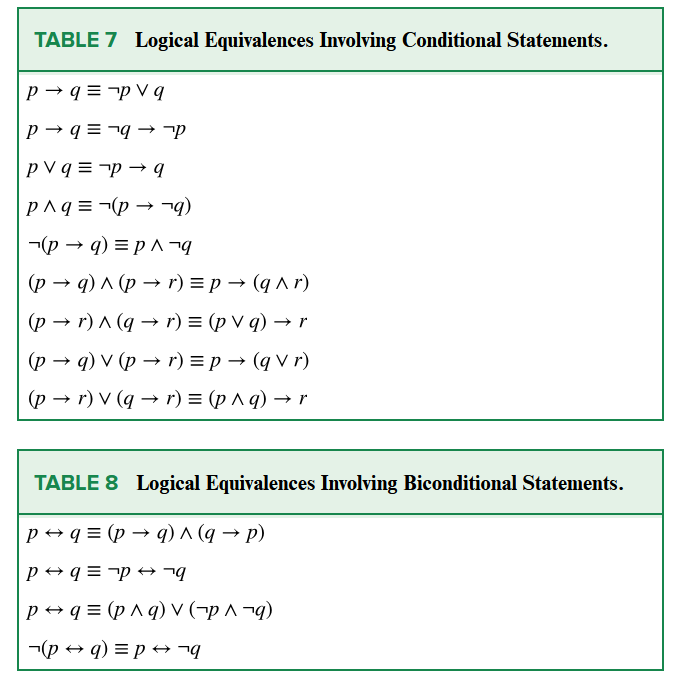
\includegraphics[width=0.72\textwidth]{1.3.D2.PNG}

\end{center}
Credit: Rosen's Discrete Mathematics 8e

When using De Morgan's Laws, remember to change the logical connective after you negate. 

De Morgan's Laws tell us how to negate conjunctions and how to negate disjunctions. 
The equivalence $\neg(p\lor q)\equiv \neg p \land \neg q$ tells us that the negation of a disjunction 
is formed from the conjunction of the negations of the component propositions. The negation of a conjunction 
also gives you the disjunction of the negations of component propositions.

A compound proposition is satisfiable if there is an assignment of truth values to its variables that make it true. 
If no such assignments exist, then it is unsatisfiable. 

\section{Predicates and Quantifiers}
We will introduce predicate logic now. For example in the statement $x$ is greater than 3, the variable is $x$ and 
the predicate is "is greater than 3".

In general a statement involving $n$ variables $x_1,x_2,\cdots,x_n$ can be denoted as $P(x_1,x_2,\cdots,x_n)$. 

\begin{definition}
    The universal quantification of $P(x)$ is the statement:

    "$P(x)$ for all values of $x$ in the domain."

    The notation $\forall x P(x)$ denotes the universal quantification of $P(x)$. Here $\forall$ 
    is called the universal quantifier. An element for which $P(x)$ is false is called a counterexample to $\forall x P(x)$.
\end{definition}

\begin{definition}
    The existential quantification of $P(x)$ is the proposition:

    "There exists an element in $x$ in the domain such that $P(x)$"

    We use the notation $\exists x P(x)$ for the existential quantification of $P(x)$.
\end{definition}

Remember the truth value for both $\forall x P(x)$ and $\exists x P(x)$ depends on the domain.
\begin{center}
    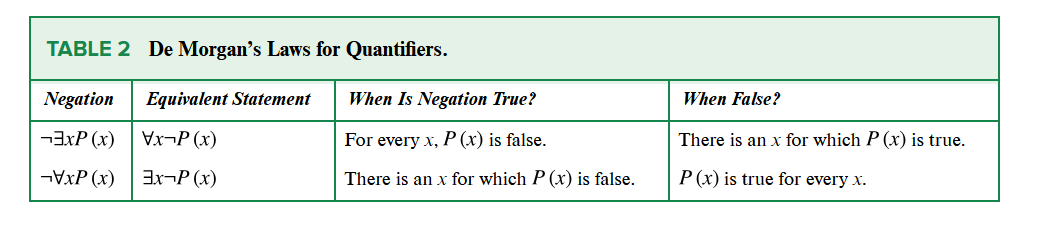
\includegraphics[width=0.9\textwidth]{1.4.PNG}
\end{center}
Credit: Rosen's Discrete Mathematics 8e

\section{Nested Quantifiers}
A nested quantifier is when one quantifier is in the scope of another.

Here is table that summarizes different quantifications involving two variables.
\begin{center}
    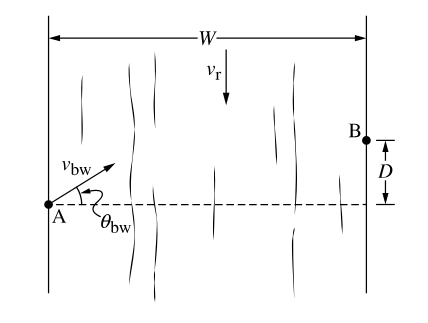
\includegraphics[width=1\textwidth]{1.5.PNG}
\end{center}

\section{Rules of Inference}
Rules of inference are our basic tools for establishing the truth of statements.

An argument in propositional logic is a sequence of propositions. All but the final proposition in the 
argument are called premises and the final proposition is called the conclusion. An argument is valid 
if the truth of all its premises implies the conclusion is true.

An argument form in propositional logic is a sequence of compound propositions involving propositional 
variables. An argument form is valid if no matter what particular propositions are substituted for the 
propositional variables in the premises, the conclusion is true if the premises are all true.

The tautology $(p\land(p\rightarrow q))\rightarrow q$ is the basis of the rule of inference 
modus ponens, or the law of detachment, basically: if $p$ and $p\rightarrow q \therefore q$.

Yet again another chart I took from Rosen.
\begin{center}
    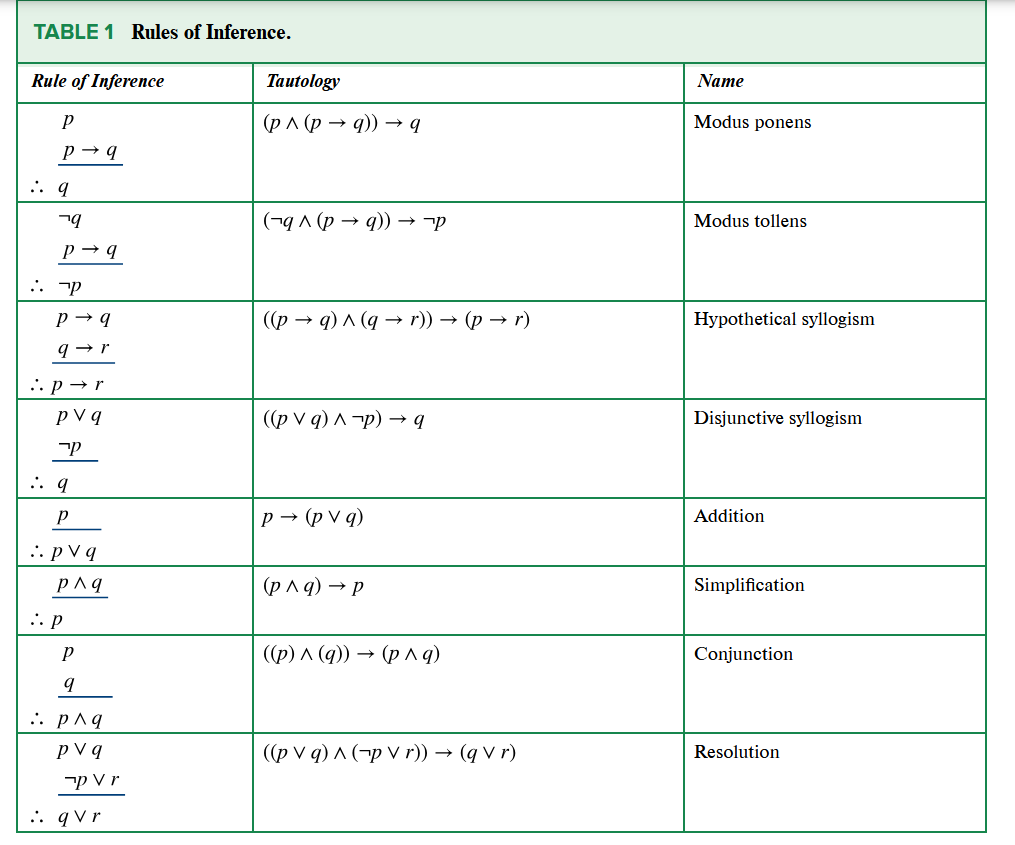
\includegraphics[width=1\textwidth]{1.6.PNG}
\end{center}

Fallacies resemble rules of inference, the difference lies in that they are based in contingencies rather than tautologies.

There are also some rules of inference for statements involving quantifiers.
This is what Rosen summarized:
\begin{center}
    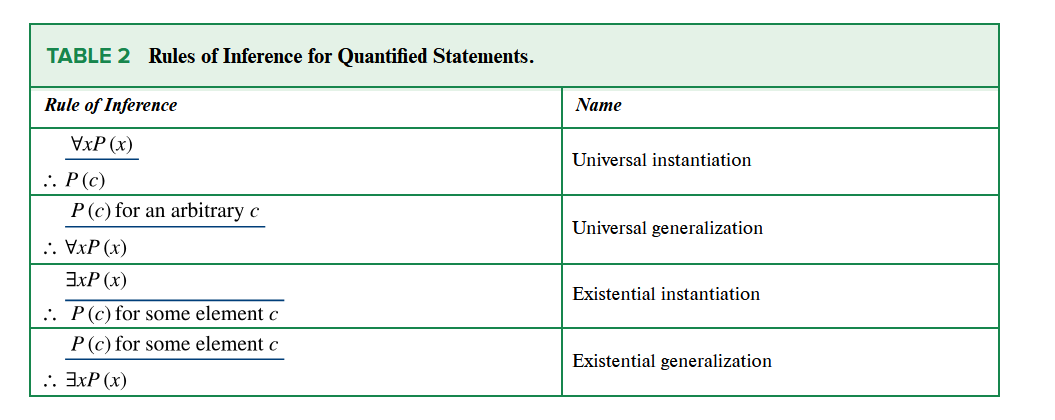
\includegraphics[width=1\textwidth]{1.6.1.PNG}
\end{center}

Because universal instantiation and modus ponens are so often used together, the combination of rules 
is called universal modus ponens. This rule tells us if $\forall x (P(x)\rightarrow Q(x))$ is true, 
and if $P(a)$ is true for a particular element $a$ in the domain of the universal quantifier, 
then $Q(a)$ must also be true. Note that by universal instantiation $P(a)\rightarrow Q(a)$ is true. 
By modus ponens, $Q(a)$ must also be true. 

This is how it is described:
\begin{center}
    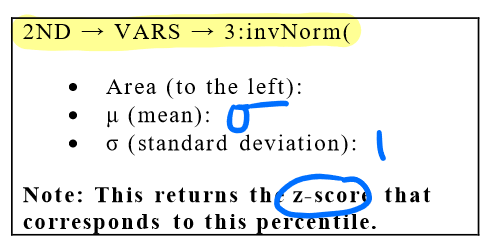
\includegraphics[width=0.5\textwidth]{1.6.2.PNG}
\end{center}

There is also universal modus tollens:
\begin{center}
    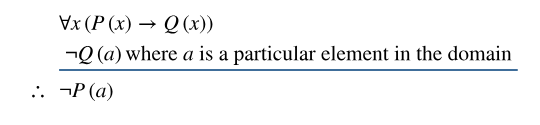
\includegraphics[width=0.5\textwidth]{1.6.3.PNG}
\end{center}

\section{Introduction to Proofs}
A proof is a valid argument that establishes the truth of a mathematical statement. 

A theorem is a statement that can be shown to be true. We show the truth using a proof.

A less important theorem that is helpful in the proof of other results is called a lemma. 

A corollary is a theorem that can be established directly from a theorem that has been proved. 

A conjecture is a statement that is being proposed to be a true statement.

A direct proof of a conditional statement $p\rightarrow q$ is constructed with the 
assumption that $p$ is true with the goal for the combination of $p$ being true and $q$ being false to never happen. 
\begin{definition}
    The integer $n$ is even if there exists an integer $k$ such that $n=2k$, and $n$ is odd if there exists an 
    integer $k$ such that $n=2k+1$. Two integers have the same parity when both are even or both are odd; they have 
    opposite parity when one is even and the other is odd.
\end{definition}

An indirect proof is a type of proof that is not direct. One example is proof by contraposition. P
roofs by contraposition use the fact that $p\rightarrow q$ is equal to $\neg q \rightarrow \neg p$. 
We have to show $\neg q \rightarrow \neg p$ is true to show that $p\rightarrow q$ is true as well.

We can prove that $p\rightarrow q$ is true if $p$ is false as well. This is called a vacuous proof. 

If we show that $q$ is true in $p\rightarrow q$ this is called a trivial proof. 
\begin{definition}
    The real number $r$ is rational if there exist integers $p$ and $q$ with $q\neq 0$ such that $r=p/q$. 
    A real number that is not rational is irrational.
\end{definition}

Suppose we want to prove a statement $p$ is true. Suppose that we can find a contradiction $q$ such that 
$\neg p \rightarrow q$ is true. Because $q$ is false, but $\neg p \rightarrow q$ is true, we can conclude 
$\neg p$ is false, meaning $p$ is true. 

To find a contradiction $q$ that might help us find that $p$ is true, we can show that 
$\neg p \rightarrow (r\land \neg r)$ is true for some proposition $r$. This is called a proof by contradiction. 

To prove a theorem in the form $p\leftrightarrow q$, we show that both $p\rightarrow q$ and $q\rightarrow p$ are both true. 

Many incorrect arguments are based on a fallacy called begging the question or circular reasoning. 
This fallacy occurs when one or more steps of a proof are based on the truth of the statement being proved.

\section{Proof Methods and Strategy}
Suppose we have a conditional $(p_1\lor p_2\lor \cdots \lor p_n)\rightarrow q$. We can separate the 
proof into different cases, called proof by cases by proving each of the $n$ conditional statements.

Some theorems can be proved by examining a relatively small number of examples. This is called proof by exhaustion. 

The phrase "without loss of generality" (WLOG) means that we assert by proving one case of a theorem, 
no additional argument is required to prove other specified cases. 

Many theorems are assertions that objects of a particular type exist. A theorem of this type is a 
proposition in the form $\exists xP(x)$, where $P$ is a predicate. A proof of a proposition in this 
form is called an existence proof. Sometimes an existence proof can be given by finding an element $a$, 
called a witness, such that $P(a)$ is true. This existence proof is called constructive. If we prove 
$\exists xP(x)$ is true in another way it can be nonconstructive.

For a uniqueness proof, we need two parts:
\begin{itemize}
    \item Existence: We show that an element $x$ with the desired property exists.
    \item Uniqueness: We show that if $x$ and $y$ both have the desired property, $x=y$
\end{itemize}

Forward reasoning is a proof when you start with your premises. You construct a proof with steps 
leading to the conclusion. It may sometimes be helpful to use backwards reasoning, we find a 
statement $p$ that we can prove $p\rightarrow q$. 
\end{document}